\subsection{Gtransfo\-Lin\-Scale  Class Reference}
\label{class_gtransfolinscale}\index{GtransfoLinScale@{Gtransfo\-Lin\-Scale}}
just here to provide specialized constructors. {\bf Gtransfo\-Lin} {\rm (p.\,\pageref{class_gtransfolin})} fit routine. 


{\tt \#include $<$gtransfo.h$>$}

Inheritance diagram for Gtransfo\-Lin\-Scale::\begin{figure}[H]
\begin{center}
\leavevmode
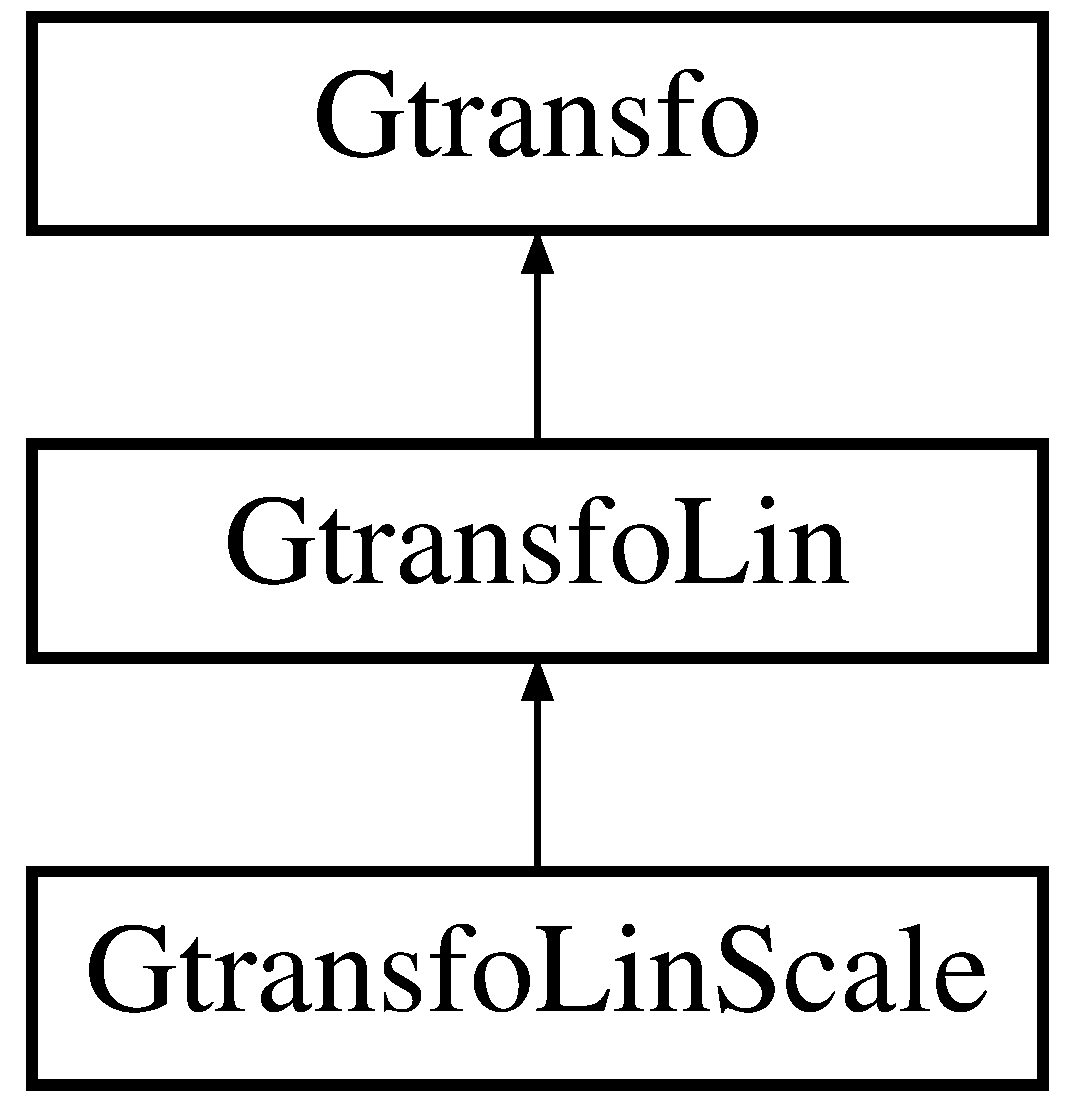
\includegraphics[height=3cm]{class_gtransfolinscale}
\end{center}
\end{figure}
\subsubsection*{Public Methods}
\begin{CompactItemize}
\item 
\index{GtransfoLinScale@{GtransfoLinScale}!GtransfoLinScale@{Gtransfo\-Lin\-Scale}}\index{GtransfoLinScale@{GtransfoLinScale}!GtransfoLinScale@{Gtransfo\-Lin\-Scale}}
{\bf Gtransfo\-Lin\-Scale} (const double Scale)\label{class_gtransfolinscale_a0}

\item 
\index{GtransfoLinScale@{GtransfoLinScale}!GtransfoLinScale@{Gtransfo\-Lin\-Scale}}\index{GtransfoLinScale@{GtransfoLinScale}!GtransfoLinScale@{Gtransfo\-Lin\-Scale}}
{\bf Gtransfo\-Lin\-Scale} (const double Scale\-X, const double Scale\-Y)\label{class_gtransfolinscale_a1}

\item 
\index{Npar@{Npar}!GtransfoLinScale@{Gtransfo\-Lin\-Scale}}\index{GtransfoLinScale@{GtransfoLinScale}!Npar@{Npar}}
int {\bf Npar} () const\label{class_gtransfolinscale_a2}

\begin{CompactList}\small\item\em returns the number of parameters (to compute chi2's).\item\end{CompactList}\end{CompactItemize}


\subsubsection{Detailed Description}
just here to provide specialized constructors. {\bf Gtransfo\-Lin} {\rm (p.\,\pageref{class_gtransfolin})} fit routine.



The documentation for this class was generated from the following file:\begin{CompactItemize}
\item 
{\bf gtransfo.h}\end{CompactItemize}
